\subsubsection{}
\paragraph*{}
Les graphiques qui vont suivre ont été généré avec une distribution
 $SBM(500,2,[0.5,0.5],a/500,b/500)$
\begin{figure}[H]
    \centering
    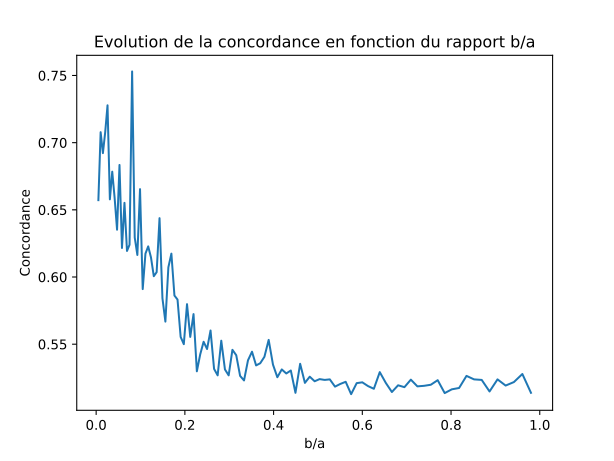
\includegraphics[width=0.6\textwidth]{figs/concordance_a_b.png}
    \caption{Evolution de la concordance en fonction du rapport $b/a$}
\end{figure}
\paragraph*{}
Ce graphique montre bien que dès que le rapport $b/a$ augmente, la concordance diminue
rapidement et tend vers $0.5$ lorque $b/a$ tend vers $1$. C'est un résultat prévisible
car plus le rapport est grand, moins il y a de communeautés de distinctes. 
\begin{figure}[H]
    \centering
    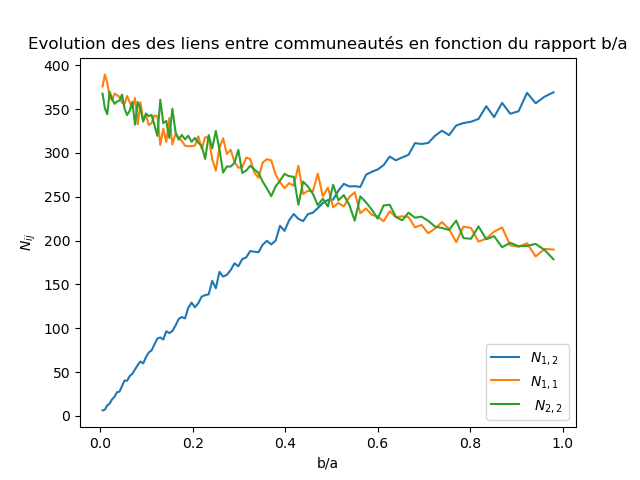
\includegraphics[width=0.6\textwidth]{figs/nij.png}
    \caption{Evolution de la concordance en fonction du rapport $b/a$}
\end{figure}
\paragraph*{}
Ce graphique nous aide a comprendre plus visuellement ce que change le rapport 
$b/a$. On remarque que plus le rapport est grand, plus il y a de liens entre les 
communautés. Quand $b/a = 0.5$, il y a autant de liens entre communautés que à 
l'intérieur des communautés. 

\paragraph*{}
En comparant les 2 graphiques, on remarque rapidement que moins les communeautes
ont de liens entre elles, plus l'algorithme de Metropolis-Hastings les détecte avec 
précisions. A partir d'un rapport $b/a = 0.2 $ notre algorithme ne donne aucun
résultats concluants

\subsubsection{}
\paragraph*{}
En considérant un degré moyen de 3 pour $\frac{a+b}{2}$, nous arrivons à ces conclusions:
\begin{align*}
    (a-b)^2 &> 2*(a+b)\\
    (a-b)^2 &> 2*12\\
    (a-b)&>\sqrt[]{24}=2*\sqrt[]{6}\\
    a&>b+2*\sqrt[]{6}\\
    a&>6-a+2*\sqrt[]{6}\\
    2*a&>6+2*\sqrt[]{6}\\
    a&>3+\sqrt[]{6}\backsimeq 5,45
\end{align*}
La condition n'est donc plus respectées pour le rapport $b/a = \frac{6-5,45}{5,45}= 0,092$